\documentclass[11pt]{article}

\usepackage{amsmath,amssymb,mathtools}
\usepackage[margin=1in]{geometry}
\usepackage{enumitem}
\usepackage{xcolor}
\usepackage{microtype}
\usepackage{graphicx}
\usepackage{tikz,float}
\usepackage{subcaption}
\usepackage{amsthm}
\usepackage{hyperref}
\usepackage{array}
\usepackage{pgfplots}

\usetikzlibrary{shapes.geometric, arrows.meta, positioning, calc, decorations.markings}
\tikzset{
	block/.style={rectangle, draw, text width=6em, text centered, rounded corners, minimum height=10mm},
	sum/.style={circle, draw, node distance=1.5cm},
	line/.style={draw, -{Stealth[length=2.5mm, width=1.5mm]}}
}

\usepgfplotslibrary{groupplots}
\pgfplotsset{compat=1.18}

\pgfplotsset{
	myaxes/.style={
		axis lines=middle,
		axis line style={-latex},
		grid=major,
		grid style={gray!15},
		minor grid style={gray!35},
		xlabel style={at={(ticklabel* cs:1)}, anchor=north west},
		ylabel style={at={(ticklabel* cs:1)}, anchor=south east},
		every axis plot/.append style={thick}
	},
	myplotstyle/.style={
		width=14cm,
		height=7cm,
		axis lines=middle,
		axis line style={-Stealth},
		grid=both,
		minor tick num=1,
		major grid style={draw=gray!30},
		minor grid style={draw=gray!15},
		tick label style={font=\small, fill=white, inner sep=1.5pt},
		xlabel={$t$},
		ylabel={$x(t)$},
		xlabel style={anchor=north east, font=\small},
		ylabel style={anchor=south east, font=\small},
		samples=401,
	}
}

\newtheoremstyle{mynote}
{6pt}      % Space above
{6pt}      % Space below
{}          % Body font (normal, not italic)
{}          % Indent amount
{\bfseries} % Theorem head font
{.}         % Punctuation after theorem head
{.5em}      % Space after theorem head
{}          % Theorem head spec
\theoremstyle{mynote}
\newtheorem{definition}{Definition}
\newtheorem{proposition}{Proposition}
\newtheorem{example}{Example}
\newtheorem{remark}{Remark}
\newtheorem{theorem}{Theorem}
\newtheorem{corollary}{Corollary}

\newcommand{\T}{\mathcal{T}}
\newcommand{\R}{\mathbb{R}}
\newcommand{\Z}{\mathbb{Z}}
\newcommand{\C}{\mathbb{C}}
\newcommand{\conv}{\ast}
\newcommand{\dt}{\,\dd t}
\newcommand{\dd}{\mathrm{d}}
\newcommand{\imp}{\delta}
\newcommand{\sinc}[1]{\frac{\sin(\pi #1)}{\pi #1}}


\DeclareMathOperator{\rect}{rect}
\DeclareMathOperator{\Ev}{Ev}
\DeclareMathOperator{\Od}{Od}
\DeclareMathOperator{\sgn}{sgn}
\DeclareMathOperator{\step}{u}
\DeclareMathOperator{\tri}{tri}



\begin{document}
	% Reset figure counter for this lecture
	\renewcommand{\thefigure}{14.\arabic{figure}}
	
	% --- TITLE BLOCK ---
	\thispagestyle{empty}
	\noindent
	\begin{tabular*}{\textwidth}{l @{\extracolsep{\fill}} r}
		\textbf{Signals and Systems} & \textbf{Lecture 14} \\
		\textit{Dr. Ghandi Manasra and Ahmed Rabei} & \textit{Fall 2025} \\
	\end{tabular*}
	\hrule
	\vspace{0.4cm}
	\begin{center}
		\Large\textbf{Lecture 14: The Discrete-Time Fourier Transform (DTFT)}
	\end{center}
	\vspace{0.4cm}
	
	\section*{Reference}
	Oppenheim \& Willsky, \textit{Signals and Systems}, Chapter 5, Sections 5.0--5.2
	
	\section*{Review of Lecture 13}
	\begin{itemize}[noitemsep]
		\item Convolution property of the CTFT
		\item LTI systems as frequency-domain multipliers
		\item Differential equations transformed to algebraic equations
		\item System frequency response analysis
	\end{itemize}
	
	\section*{14.1 Introduction}
	
	Having completed our exploration of the continuous-time frequency domain with the CTFT, we now build the parallel framework for discrete-time aperiodic signals. This leads us to the \textbf{Discrete-Time Fourier Transform (DTFT)}.
	
	The development will closely mirror our derivation of the CTFT from the CTFS. We will see strong similarities in the concepts, but also crucial differences that arise from the discrete nature of the time variable.
	
	\subsection*{14.1.1 The Core Idea:}
	
	Just as with the CTFT, we can think of an aperiodic discrete-time signal $x[n]$ as the limit of a periodic signal $\tilde{x}[n]$ as the period $N$ goes to infinity.
	
	Consider a periodic discrete-time signal $\tilde{x}[n]$ with DTFS representation:
	\[
	\tilde{x}[n] = \sum_{k=0}^{N-1} a_k e^{jk(2\pi/N)n}
	\]
	where the DTFS coefficients are:
	\[
	a_k = \frac{1}{N} \sum_{n=0}^{N-1} \tilde{x}[n]e^{-jk(2\pi/N)n}
	\]
	\newpage
	\subsection*{14.1.2 The Envelope Function:}
	
	We define an \textbf{envelope function} $X(e^{j\omega})$ by scaling the DTFS coefficients:
	\[
	X(e^{jk(2\pi/N)}) = N a_k = \sum_{n=-\infty}^{\infty} x[n]e^{-jk(2\pi/N)n}
	\]
	
	This envelope function represents the continuous frequency content for our signal.
	
	Rewriting the synthesis equation in terms of this envelope:
	\[
	\tilde{x}[n] = \sum_{k=0}^{N-1} \frac{1}{N} X(e^{jk(2\pi/N)}) e^{jk(2\pi/N)n} = \frac{1}{2\pi} \sum_{k=0}^{N-1} X(e^{jk(2\pi/N)}) e^{jk(2\pi/N)n} \left(\frac{2\pi}{N}\right)
	\]
	
	\subsection*{14.1.3 Taking the Limit:}
	
	As $N \to \infty$:
	\begin{itemize}[noitemsep]
		\item $\tilde{x}[n] \to x[n]$ - the periodic signal becomes aperiodic
		\item $\omega_0 = \frac{2\pi}{N} \to 0$ - the frequency spacing shrinks
		\item $k\omega_0$ becomes a continuous variable $\omega$ - discrete frequencies become continuous
		\item The sum becomes an integral
	\end{itemize}
	
	This leads to the \textbf{DTFT pair}:
	
	\section*{14.2 The Discrete-Time Fourier Transform (DTFT)}
	
	\begin{definition}
		For a discrete-time signal $x[n]$, the \textbf{analysis equation} (DTFT) is:
		\[
		X(e^{j\omega}) = \sum_{n=-\infty}^{\infty} x[n]e^{-j\omega n}
		\]
		The \textbf{synthesis equation} (Inverse DTFT) is:
		\[
		x[n] = \frac{1}{2\pi} \int_{2\pi} X(e^{j\omega})e^{j\omega n} \dd\omega
		\]
		The integral is over \textit{any} interval of length $2\pi$.
	\end{definition}
	
	\subsection*{14.2.1 Convergence Conditions}
	
	The DTFT converges when the discrete-time signal is absolutely summable:
	\[
	\sum_{n=-\infty}^{\infty} |x[n]| < \infty
	\]
	
	\begin{remark}
		This condition ensures that the infinite sum defining the DTFT converges to a finite, continuous function of $\omega$. For signals that don't satisfy this condition, generalized DTFT definitions may be employed.
	\end{remark}
	
\subsection*{14.2.2 Convergence Examples}
	
	\textbf{Convergent signals:}
	\begin{itemize}[noitemsep]
		\item $a^n u[n]$ for $|a| < 1$ (absolutely summable)
		\item Finite-length sequences (always absolutely summable)
		\item Signals with exponential decay
	\end{itemize}
	
	\textbf{Non-convergent signals (require generalized DTFT):}
	\begin{itemize}[noitemsep]
		\item Constant signal $x[n] = 1$ (not absolutely summable)
		\item Complex exponentials $e^{j\omega_0 n}$ (not absolutely summable)
		\item Periodic signals (not absolutely summable)
	\end{itemize}
	
\subsection*{14.2.3 The Fundamental Property: Periodicity}
	
	The most critical property of the DTFT is its \textbf{periodicity in frequency with period $2\pi$}:
	\[
	X(e^{j(\omega+2\pi)}) = \sum_{n=-\infty}^{\infty} x[n]e^{-j(\omega+2\pi)n} = \sum_{n=-\infty}^{\infty} x[n]e^{-j\omega n} \underbrace{e^{-j2\pi n}}_{=1} = X(e^{j\omega})
	\]
	
	\textbf{Intuition:} All the unique frequency information for a discrete-time signal is contained within a single $2\pi$ interval (e.g., from $-\pi$ to $\pi$). This is a direct consequence of the discrete nature of time. A discrete-time system cannot distinguish between a frequency $\omega_0$ and a frequency $\omega_0+2\pi$. This phenomenon is called \textbf{aliasing}.
	
	\begin{figure}[H]
		\centering
		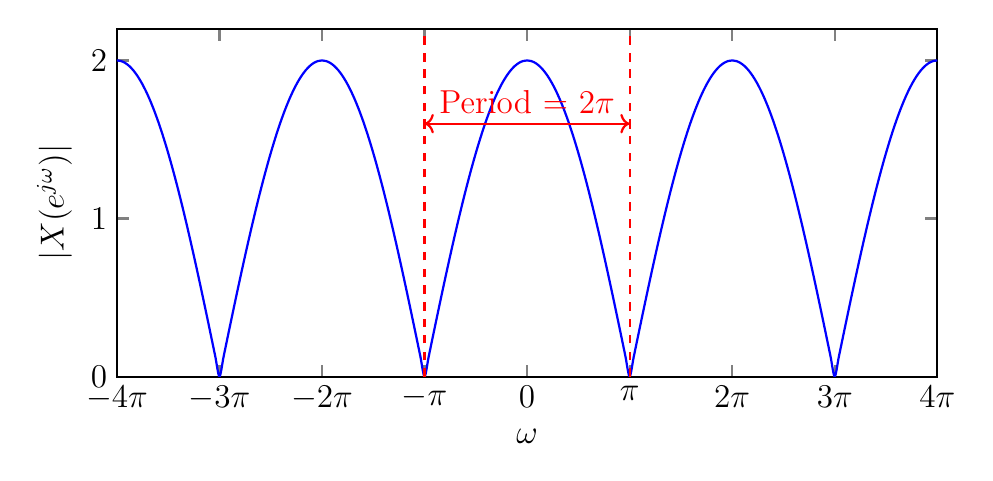
\begin{tikzpicture}
	\begin{axis}[
		width=12cm,
		height=6cm,
		xlabel={$\omega$},
		ylabel={$|X(e^{j\omega})|$},
		xmin=-4*pi, xmax=4*pi,
		ymin=0, ymax=2.2,
		xtick={-4*pi, -3*pi, -2*pi, -pi, 0, pi, 2*pi, 3*pi, 4*pi},
		xticklabels={$-4\pi$, $-3\pi$, $-2\pi$, $-\pi$, $0$, $\pi$, $2\pi$, $3\pi$, $4\pi$},
		ytick={0, 1, 2},
		domain=-4*pi:4*pi,
		samples=201,
		smooth,
		axis line style={thick},
		tick style={thick},
		label style={font=\large},
		tick label style={font=\large},
		every axis plot/.append style={thick},
		]
		% Plot the magnitude spectrum as 2*|cos(ω/2)|
		\addplot[blue] {2*abs(cos(deg(x/2)))};
		
		% Vertical dashed periodicity lines at -2π and 2π
		\addplot[red, dashed] coordinates {(-pi, 0) (-pi, 2.2)};
		\addplot[red, dashed] coordinates {(pi, 0) (pi, 2.2)};
		
		% Periodicity arrow with label above the curve
		% The non-breaking space between the coordinate and the 'node' command was replaced
		% with a regular space.
		\draw[<->, thick, red] (axis cs: -pi, 1.6) -- (axis cs: pi, 1.6)
		node[midway, above, font=\large] {Period = $2\pi$};
	\end{axis}
\end{tikzpicture}
		\caption{DTFT periodicity: The spectrum repeats every $2\pi$ radians}
		\label{fig:dtft_periodicity}
	\end{figure}
	\newpage
	\section*{14.3 Examples}
	
	\subsection*{14.3.1 Decaying Exponential}
	
	Let $x[n] = a^n u[n]$ for $|a| < 1$.
	
	\begin{align}
		X(e^{j\omega}) &= \sum_{n=0}^{\infty} a^n e^{-j\omega n} \\
		&= \sum_{n=0}^{\infty} (ae^{-j\omega})^n \\
		&= \frac{1}{1-ae^{-j\omega}}
	\end{align}
	
	\textbf{Transform pair (for $|a|<1$):} \quad $a^n u[n] \stackrel{\mathcal{F}}{\longleftrightarrow} \dfrac{1}{1-ae^{-j\omega}}$
	
	\subsection*{14.3.2 Rectangular Pulse}
	
	Let $x[n] = \begin{cases} 1, & 0 \leq n \leq N_1-1 \\ 0, & \text{otherwise} \end{cases}$.
	
	\begin{align}
		X(e^{j\omega}) &= \sum_{n=0}^{N_1-1} e^{-j\omega n} \\
		&= \frac{1 - (e^{-j\omega})^{N_1}}{1 - e^{-j\omega}} \\
		&= \frac{e^{-j\omega N_1/2}(e^{j\omega N_1/2} - e^{-j\omega N_1/2})}{e^{-j\omega/2}(e^{j\omega/2} - e^{-j\omega/2})} \\
		&= e^{-j\omega(N_1-1)/2} \frac{\sin(\omega N_1/2)}{\sin(\omega/2)}
	\end{align}
	
	This is the discrete-time counterpart of the sinc function
	
	\begin{figure}[H]
		\centering
		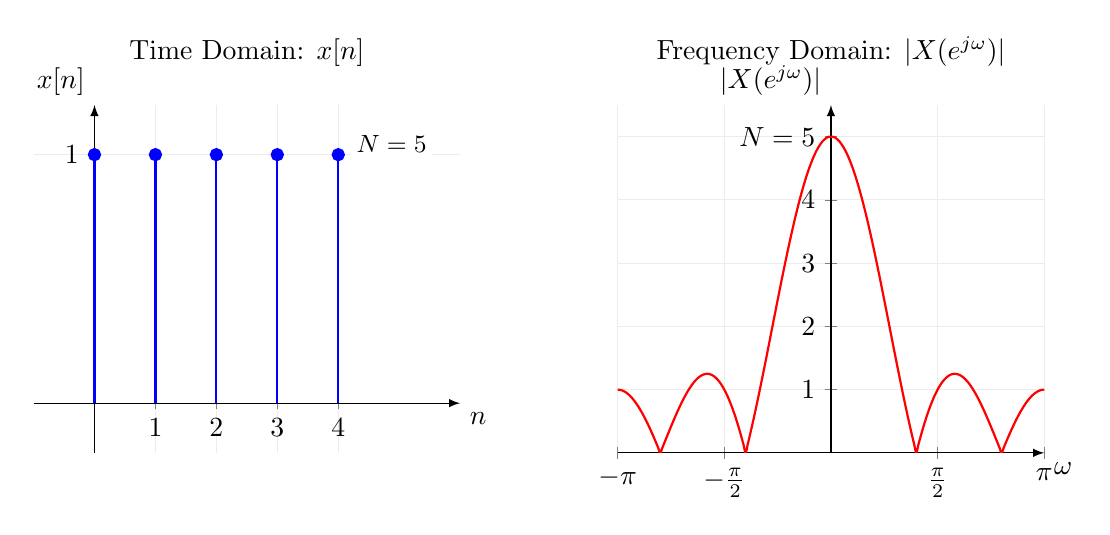
\begin{tikzpicture}
	\begin{groupplot}[
		group style={
			group size=2 by 1,
			horizontal sep=2cm,
		},
		myaxes, % Assumes this style is defined elsewhere
		width=7cm,
		height=6cm,
		title style={yshift=1ex},
		]
		
		% Subplot 1: Time Domain (Hardcoded for N=5)
		\nextgroupplot[
		title={Time Domain: $x[n]$},
		xlabel={$n$},
		ylabel={$x[n]$},
		xmin=-1, xmax=6,
		ymin=-0.2, ymax=1.2,
		xtick={0, 1, 2, 3, 4},
		ytick={0, 1},
		]
		\addplot[
		blue, thick, ycomb, mark=*, mark options={fill=blue},
		domain=0:4,
		samples=5,
		] {1};
		\node[anchor=north west, fill=white, inner sep=2pt, font=\small] at (axis cs: 4.2, 1.1) {$N = 5$};
		
		
		% Subplot 2: Frequency Domain (FIXED)
		\nextgroupplot[
		title={Frequency Domain: $|X(e^{j\omega})|$},
		xlabel={$\omega$},
		ylabel={$|X(e^{j\omega})|$},
		xmin=-pi, xmax=pi,
		ymin=0, ymax=5.5,
		xtick={-pi, -pi/2, 0, pi/2, pi},
		xticklabels={$-\pi$, $-\frac{\pi}{2}$, $0$, $\frac{\pi}{2}$, $\pi$},
		ytick={0, 1, 2, 3, 4, 5},
		yticklabels={0, 1, 2, 3, 4, {$N=5$}},
		domain=-pi:pi,
		samples=201,
		]
		% --- THIS IS THE CORRECTED LINE ---
		\addplot[red, thick, smooth] {
			% Use a ternary operator to handle the case at x=0
			abs(x) < 0.001 ? 5 : abs(sin(deg(5*x/2))/sin(deg(x/2)))
		};
		
	\end{groupplot}
\end{tikzpicture}
		\caption{Rectangular pulse and its DTFT}
		\label{fig:rectangular_pulse_dtft}
	\end{figure}
	
	\subsection*{14.3.3 Unit Impulse}
	
	Let $x[n] = \delta[n]$.
	
	The sum has only one non-zero term at $n=0$:
	\[
	X(e^{j\omega}) = \sum_{n=-\infty}^{\infty} \delta[n]e^{-j\omega n} = 1 \cdot e^{-j\omega \cdot 0} = 1
	\]
	
	\textbf{Transform pair:} \quad $\delta[n] \stackrel{\mathcal{F}}{\longleftrightarrow} 1$
	
	\textbf{Intuition:} Just like its continuous-time counterpart, the discrete-time impulse contains equal energy at all frequencies within the unique $2\pi$ interval.
	
	\subsection*{14.3.4 Constant Signal}
	
	Let $x[n] = 1$ for all $n$.
	
	This signal is not absolutely summable, so its DTFT cannot be found by direct evaluation. Instead, we work backward from the synthesis equation.
	
	Let's propose that the transform of $x[n] = 1$ is a scaled Dirac delta function, $X(e^{j\omega}) = c\delta(\omega)$, and find the constant $c$.
	\[
	x[n] = \frac{1}{2\pi} \int_{2\pi} c\delta(\omega)e^{j\omega n} \dd\omega
	\]
	
	Using the sifting property:
	\[
	x[n] = \frac{c}{2\pi} e^{j(0)n} = \frac{c}{2\pi}
	\]
	
	We want this result to be equal to our original signal, $x[n] = 1$. Therefore:
	\[
	\frac{c}{2\pi} = 1 \implies c = 2\pi
	\]
	
	\textbf{Verification:} Let's verify this works by substituting back into the synthesis equation:
	\[
	x[n] = \frac{1}{2\pi} \int_{2\pi} 2\pi\delta(\omega)e^{j\omega n} \dd\omega = \int_{2\pi} \delta(\omega)e^{j\omega n} \dd\omega = e^{j(0)n} = 1
	\]
	
	This gives us the transform pair:
	\[
	1 \stackrel{\mathcal{F}}{\longleftrightarrow} 2\pi\sum_{k=-\infty}^{\infty} \delta(\omega - 2\pi k)
	\]
	
	\begin{remark}
		The DTFT of a constant signal is a periodic train of impulses with period $2\pi$. The expression $2\pi\delta(\omega)$ represents only the $k=0$ impulse in this train, valid over a single period like $[-\pi, \pi)$.
	\end{remark}
	\newpage
	\subsection*{14.3.5 Complex Exponential}
	
	Let $x[n] = e^{j\omega_0 n}$.
	
	Using the same method as for a constant signal, we propose that the transform is $X(e^{j\omega}) = c\delta(\omega - \omega_0)$ and find the constant $c$.
	\[
	x[n] = \frac{1}{2\pi} \int_{2\pi} c\delta(\omega - \omega_0)e^{j\omega n} \dd\omega
	\]
	
	Using the sifting property:
	\[
	x[n] = \frac{c}{2\pi} e^{j\omega_0 n}
	\]
	
	We want this result to be equal to our original signal, $x[n] = e^{j\omega_0 n}$. Therefore:
	\[
	\frac{c}{2\pi} = 1 \implies c = 2\pi
	\]
	
	\textbf{Verification:} Let's verify this works by substituting back into the synthesis equation:
	\[
	x[n] = \frac{1}{2\pi} \int_{2\pi} 2\pi\delta(\omega - \omega_0)e^{j\omega n} \dd\omega = \int_{2\pi} \delta(\omega - \omega_0)e^{j\omega n} \dd\omega = e^{j\omega_0 n}
	\]
	
	This gives us the transform pair:
	\[
	e^{j\omega_0 n} \stackrel{\mathcal{F}}{\longleftrightarrow} 2\pi\sum_{k=-\infty}^{\infty} \delta(\omega - \omega_0 - 2\pi k)
	\]
	
	\begin{remark}
		The DTFT of a complex exponential is a periodic train of impulses with period $2\pi$. The expression $2\pi\delta(\omega - \omega_0)$ represents only the $k=0$ impulse in this train, valid over a single period like $[-\pi, \pi)$.
	\end{remark}
	
	\subsection*{14.3.6 Sinusoidal Signals}
	
	For $x[n] = \sin(\omega_0 n)$:
	
	Using Euler's identity: $\sin(\omega_0 n) = \frac{1}{2j}(e^{j\omega_0 n} - e^{-j\omega_0 n})$
	\[
	\sin(\omega_0 n) = \frac{1}{2j}e^{j\omega_0 n} - \frac{1}{2j}e^{-j\omega_0 n}
	\]
	
	Using linearity and the complex exponential result:
	\[
	\sin(\omega_0 n) \stackrel{\mathcal{F}}{\longleftrightarrow} \frac{1}{2j} \cdot 2\pi\sum_{k=-\infty}^{\infty} \delta(\omega - \omega_0 - 2\pi k) - \frac{1}{2j} \cdot 2\pi\sum_{k=-\infty}^{\infty} \delta(\omega + \omega_0 - 2\pi k)
	\]
	\[
	\sin(\omega_0 n) \stackrel{\mathcal{F}}{\longleftrightarrow} j\pi\sum_{k=-\infty}^{\infty} [\delta(\omega + \omega_0 - 2\pi k) - \delta(\omega - \omega_0 - 2\pi k)]
	\]
	
	For $x[n] = \cos(\omega_0 n)$:
	
	Using Euler's identity: $\cos(\omega_0 n) = \frac{1}{2}(e^{j\omega_0 n} + e^{-j\omega_0 n})$
	\[
	\cos(\omega_0 n) = \frac{1}{2}e^{j\omega_0 n} + \frac{1}{2}e^{-j\omega_0 n}
	\]
	
	Using linearity and the complex exponential result:
	\[
	\cos(\omega_0 n) \stackrel{\mathcal{F}}{\longleftrightarrow} \frac{1}{2} \cdot 2\pi\sum_{k=-\infty}^{\infty} \delta(\omega - \omega_0 - 2\pi k) + \frac{1}{2} \cdot 2\pi\sum_{k=-\infty}^{\infty} \delta(\omega + \omega_0 - 2\pi k)
	\]
	\[
	\cos(\omega_0 n) \stackrel{\mathcal{F}}{\longleftrightarrow} \pi\sum_{k=-\infty}^{\infty} [\delta(\omega + \omega_0 - 2\pi k) + \delta(\omega - \omega_0 - 2\pi k)]
	\]
	
	\begin{figure}[H]
		\centering
		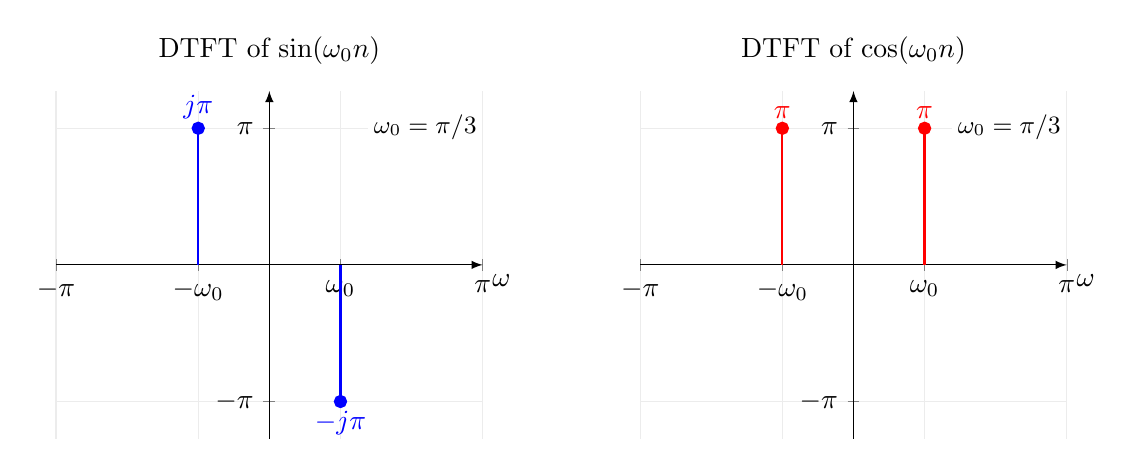
\begin{tikzpicture}
	% Define omega_0 for consistency
	\pgfmathsetmacro{\wO}{pi/3}
	
	\begin{groupplot}[
		group style={
			group size=2 by 1,
			horizontal sep=2cm,
		},
		myaxes, % Assumes this style is defined in your preamble
		width=7cm,
		height=6cm,
		xlabel={$\omega$},
		xmin=-pi, xmax=pi,
		ymin=-4, ymax=4,
		xtick={-pi, -\wO, 0, \wO, pi},
		xticklabels={$-\pi$, $-\omega_0$, $0$, $\omega_0$, $\pi$},
		ytick={-pi, 0, pi},
		yticklabels={$-\pi$, 0, $\pi$},
		]
		
		% Subplot 1: DTFT of sin(ω₀n) -> PLOTS IMAGINARY PART
		\nextgroupplot[
		title={DTFT of $\sin(\omega_0 n)$},
		]
		
		% Impulse at -ω₀ has amplitude +jπ
		\addplot[blue, thick, ycomb, mark=*, mark options={fill=blue}] coordinates {(-\wO, pi)};
		% Impulse at +ω₀ has amplitude -jπ
		\addplot[blue, thick, ycomb, mark=*, mark options={fill=blue}] coordinates {(\wO, -pi)};
		
		% Add labels
		\node[anchor=south, blue] at (axis cs: -\wO, pi) {$j\pi$};
		\node[anchor=north, blue] at (axis cs: \wO, -pi) {$-j\pi$};
		\node[anchor=north east, fill=white, inner sep=2pt, font=\small] at (axis description cs: 1, 0.95) {$\omega_0 = \pi/3$};
		
		
		% Subplot 2: DTFT of cos(ω₀n) -> PLOTS REAL PART
		\nextgroupplot[
		title={DTFT of $\cos(\omega_0 n)$},
		]
		
		% Impulse at -ω₀ has amplitude +π
		\addplot[red, thick, ycomb, mark=*, mark options={fill=red}] coordinates {(-\wO, pi)};
		% Impulse at +ω₀ has amplitude +π
		\addplot[red, thick, ycomb, mark=*, mark options={fill=red}] coordinates {(\wO, pi)};
		
		% Add labels
		\node[anchor=south, red] at (axis cs: -\wO, pi) {$\pi$};
		\node[anchor=south, red] at (axis cs: \wO, pi) {$\pi$};
		\node[anchor=north east, fill=white, inner sep=2pt, font=\small] at (axis description cs: 1, 0.95) {$\omega_0 = \pi/3$};
		
	\end{groupplot}
\end{tikzpicture}
		\caption{DTFT of sinusoidal signals: (a) $\sin(\omega_0 n)$, (b) $\cos(\omega_0 n)$}
		\label{fig:sinusoidal_dtft}
	\end{figure}
	\newpage
	\section*{14.4 Spectrum and Frequency Content}
	
	The DTFT $X(e^{j\omega})$ represents the \textbf{spectrum} of the signal $x[n]$, showing how the signal's energy is distributed across different frequencies.
	
	\begin{itemize}[noitemsep]
		\item \textbf{Magnitude spectrum} $|X(e^{j\omega})|$: Shows the strength of each frequency component
		\item \textbf{Phase spectrum} $\angle X(e^{j\omega})$: Shows the phase relationship of each frequency component
	\end{itemize}
	
	\subsection*{14.4.1 Symmetry Properties}
	
	For real-valued signals $x[n]$, the DTFT exhibits important symmetry properties:
	
	\textbf{Conjugate symmetry (real signals):} If $x[n]$ is real, then $X(e^{-j\omega}) = X^*(e^{j\omega})$.
	
	\textbf{Consequences:}
	\begin{itemize}[noitemsep]
		\item \textbf{Magnitude spectrum is even:} $|X(e^{-j\omega})| = |X(e^{j\omega})|$
		\item \textbf{Phase spectrum is odd:} $\angle X(e^{-j\omega}) = -\angle X(e^{j\omega})$
		\item \textbf{Real part is even:} $\text{Re}\{X(e^{-j\omega})\} = \text{Re}\{X(e^{j\omega})\}$
		\item \textbf{Imaginary part is odd:} $\text{Im}\{X(e^{-j\omega})\} = -\text{Im}\{X(e^{j\omega})\}$
	\end{itemize}
	
	\section*{14.5 Parseval's Theorem and Energy Conservation}
	
	\begin{theorem}[Parseval's Theorem]
		For a signal $x[n]$ with DTFT $X(e^{j\omega})$:
		\[
		\sum_{n=-\infty}^{\infty} |x[n]|^2 = \frac{1}{2\pi} \int_{2\pi} |X(e^{j\omega})|^2 \dd\omega
		\]
	\end{theorem}
	
	This result states that the total energy in a signal is the same whether calculated in the time domain or frequency domain. The quantity $|X(e^{j\omega})|^2$ is called the \textbf{energy spectral density}.
	
	\section*{14.6 Relationship to Continuous-Time Fourier Transform}
	
	The DTFT serves as the discrete-time equivalent of the continuous-time Fourier transform (CTFT), but with key differences:
	
	\begin{enumerate}[noitemsep]
		\item \textbf{Domain}: CTFT maps continuous-time signals to aperiodic frequency functions; DTFT maps discrete-time signals to periodic frequency functions
		\item \textbf{Mathematical form}: CTFT uses integrals; DTFT uses summations
		\item \textbf{Frequency range}: CTFT spans $(-\infty, \infty)$; DTFT is meaningful only over $[0, 2\pi)$ due to periodicity
	\end{enumerate}
	
	\section*{14.7 Practice Problems and Examples}
	
	\subsection*{14.7.1 Solved Example}
	
	\begin{example}
		Find the DTFT of $x[n] = a^{|n|}$ for $|a| < 1$.
		
		\textbf{Solution:} We can split the sum into two parts:
		\[
		X(e^{j\omega}) = \sum_{n=-\infty}^{\infty} a^{|n|} e^{-j\omega n} = \sum_{n=0}^{\infty} a^n e^{-j\omega n} + \sum_{n=-\infty}^{-1} a^{-n} e^{-j\omega n}
		\]
		
		The first part is a standard geometric series:
		\[
		\sum_{n=0}^{\infty} a^n e^{-j\omega n} = \sum_{n=0}^{\infty} (ae^{-j\omega})^n = \frac{1}{1-ae^{-j\omega}}
		\]
		
		For the second part, let $m = -n$:
		\[
		\sum_{n=-\infty}^{-1} a^{-n} e^{-j\omega n} = \sum_{m=1}^{\infty} a^m e^{j\omega m} = \sum_{m=1}^{\infty} (ae^{j\omega})^m = \frac{ae^{j\omega}}{1-ae^{j\omega}}
		\]
		
		Adding these two terms and simplifying:
		\[
		X(e^{j\omega}) = \frac{1}{1-ae^{-j\omega}} + \frac{ae^{j\omega}}{1-ae^{j\omega}} = \frac{1-a^2}{1-2a\cos(\omega)+a^2}
		\]
	\end{example}
	
	\subsection*{14.7.2 Practice Exercises}
	
	\begin{enumerate}[noitemsep]
		\item Find the DTFT of $x[n] = \delta[n-n_0]$.
		
		\textbf{Solution:} $X(e^{j\omega}) = e^{-j\omega n_0}$
		
		\item Find the DTFT of $x[n] = u[n] - u[n-N]$.
		
		\textbf{Solution:} This is a rectangular pulse of length $N$. Using the result from Section 14.3.2:
		$X(e^{j\omega}) = e^{-j\omega(N-1)/2} \frac{\sin(\omega N/2)}{\sin(\omega/2)}$
		
		\item Using Parseval's theorem, find the energy of $x[n] = a^n u[n]$ for $|a| < 1$.
		
		\textbf{Solution:} $E = \sum_{n=0}^{\infty} |a|^{2n} = \frac{1}{1-|a|^2}$
		
		\item Find the DTFT of $x[n] = n a^n u[n]$ for $|a| < 1$.
		
		\textbf{Solution:} $X(e^{j\omega}) = \frac{ae^{-j\omega}}{(1-ae^{-j\omega})^2}$
		
		\item Show that if $x[n]$ is real, then $X(e^{-j\omega}) = X^*(e^{j\omega})$.
		
		\textbf{Solution:} $X(e^{-j\omega}) = \sum_{n=-\infty}^{\infty} x[n]e^{j\omega n} = \left(\sum_{n=-\infty}^{\infty} x[n]e^{-j\omega n}\right)^* = X^*(e^{j\omega})$
	\end{enumerate}
	
\section*{14.8 Summary and Next Lecture}
	
	The Discrete-Time Fourier Transform extends our frequency-domain analysis to aperiodic discrete-time signals:
	
	\textbf{Key Takeaways:}
	\begin{itemize}[noitemsep]
		\item \textbf{The DTFT emerges naturally from the DTFS as the period approaches infinity}
		\item \textbf{The analysis equation $X(e^{j\omega}) = \sum_{n=-\infty}^{\infty} x[n]e^{-j\omega n}$ extracts frequency content}
		\item \textbf{The synthesis equation $x[n] = \frac{1}{2\pi} \int_{2\pi} X(e^{j\omega})e^{j\omega n} \dd\omega$ reconstructs the signal}
		\item \textbf{The spectrum $X(e^{j\omega})$ is always periodic with period $2\pi$}
		\item \textbf{Convergence is guaranteed by absolute summability for most practical signals}
		\item \textbf{The periodicity property has profound implications for digital signal processing}
		\item \textbf{Next time:} Properties of the DTFT and discrete-time LTI analysis
	\end{itemize}
\end{document}
